% =====================================================================
%  LLM-Aided Evolutionary Optimisation for Emotion-Aware, Form-Constrained
%  Poem Generation: A GA vs NSGA-II Study
%
%  ACM sigconf format (the format used by GECCO Companion papers).
%  `nonacm` removes the ACM copyright / reference-format block, because this
%  is a manuscript and has no conference, DOI or ISBN yet. When a venue
%  accepts it: delete `nonacm`, then add the \acmConference, \acmDOI and
%  \acmISBN lines the venue gives you.
%  Build: pdflatex gecco && bibtex gecco && pdflatex gecco && pdflatex gecco
% =====================================================================
\documentclass[sigconf,nonacm]{acmart}

\usepackage{booktabs}
\usepackage{tikz}
\usetikzlibrary{arrows.meta,calc,positioning,fit}
\newcommand{\Qb}{\bar{Q}}
\settopmatter{printacmref=false}

\begin{document}

\title{LLM-Aided Evolutionary Optimisation for Emotion-Aware, Form-Constrained Poem Generation: A GA vs NSGA-II Study}

\author{Sakthi C R}
\affiliation{%
  \position{M.Tech Artificial Intelligence}
  \department{Amrita School of Computing}
  \institution{Amrita Vishwa Vidyapeetham}
  \city{Coimbatore}
  \country{India}}

\author{Bagavathi C.}
\affiliation{%
  \position{Assistant Professor (Sr. Gd.)}
  \department{Department of Computer Science and Engineering, Amrita School of Computing}
  \institution{Amrita Vishwa Vidyapeetham}
  \city{Coimbatore}
  \country{India}}

\begin{abstract}
Language models are now routinely placed inside evolutionary loops, acting both as the variation operator and as the fitness judge, yet systems of this kind usually adopt a multi-objective algorithm without comparing it to a simple baseline. We run that ablation for haiku and limerick generation. An elitist single-objective genetic algorithm (GA) and NSGA-II share one pipeline --- the same generator, judge, fitness terms, population size, mutation scheme and stopping rule --- and are compared over twelve conditions (two forms $\times$ three emotions $\times$ two algorithms). The result is null: mean final fitness is 0.8368 for the GA and 0.8358 for NSGA-II, a gap of 0.0010. Auditing the fitness function explains why. The LLM judge separates deliberately bad poems from published human ones ($p=0.005$ for haiku, $0.001$ for limericks) but is unstable: 39 of 53 poems changed score between identical readings, contributing $\pm0.022$ to fitness, about twenty times the effect under study. We report this noise budget and the measurement protocol that follows from it.
\end{abstract}

\keywords{evolutionary algorithms, NSGA-II, large language models, poetry generation, LLM-as-a-judge, measurement validity}

\maketitle

% =====================================================================
\section{Introduction}
% =====================================================================
A haiku must fit a 5-7-5 syllable frame and still carry an image and a mood; a limerick must follow an AABBA rhyme scheme and a bouncing line length while telling a small story. Instruction-tuned language models write fluent verse in seconds, but a single pass rarely meets form, rhyme and emotion together. A common remedy wraps the model in an evolutionary loop in which it mutates its own output and a second model scores the candidates \cite{lehman2022,meyerson2024,bradley2024}. The LLM-aided haiku generator of Jobanputra et al.\ \cite{jobanputra2025} is one example, evolving haiku with NSGA-II on emotion and rhyme objectives.

What is missing is a control. To our knowledge, systems of this kind do not report what a simple single-objective genetic algorithm (GA) would have produced from the same generator, judge and budget, so the contribution of the search algorithm cannot be separated from that of the language model doing the writing. We run that ablation and then ask whether the instrument could have detected a difference at all. Our research questions are:
\begin{enumerate}
\item[\textbf{RQ1}] With generator, judge, fitness terms, budget and stopping rule fixed, does NSGA-II produce better poems than an elitist GA?
\item[\textbf{RQ2}] Can the LLM judge that serves as fitness function discriminate poem quality, and what bias does it show?
\item[\textbf{RQ3}] How large is its measurement noise relative to the difference between the algorithms?
\end{enumerate}
Our contributions are a controlled GA-versus-NSGA-II ablation over two forms and three emotions with every run logged; a validation of the judge against published human poems and deliberately bad controls on one scale; and a measured noise budget for the fitness function, with the protocol that follows from it.

% =====================================================================
\section{Background}
% =====================================================================
Language models as variation operators were introduced for code by Lehman et al.\ \cite{lehman2022}, generalised by prompting with several parents \cite{meyerson2024}, and applied to prompt search \cite{guo2024} and program search \cite{romera2024}; Wu et al.\ \cite{wu2025survey} survey the area, and quality-diversity through AI feedback \cite{bradley2024} used a model both to vary texts, poems included, and to judge them. Across this literature the search algorithm is typically chosen rather than compared. For poetry, genetic algorithms predate LLMs \cite{manurung2012}, and Koziev and Sinev \cite{koziev2026} survey generation and evaluation. Evaluation is the harder half: non-expert readers cannot reliably tell model poems from human ones and tend to prefer the former \cite{porter2024}, whereas LLM-written stories fall short of expert-written ones on a structured creativity test \cite{chakrabarty2024}. LLM judges agree with human preference at about the level humans agree with each other, but show position, verbosity and self-enhancement biases \cite{zheng2023}, and presentation order alone can change a verdict \cite{wang2024fair}. Judge scores are therefore noisy measurements, not ground truth; what is rarely done is to propagate that noise into the conclusions.

% =====================================================================
\section{Method}
% =====================================================================
\textbf{Pipeline.} A user gives a poem type, an emotion and a one-sentence scenario. A generator model writes a population of six poems, every candidate is scored, the algorithm under test selects a parent, and the generator rewrites that parent into five variants. The loop stops when the tracked best fitness improves by less than $0.01$ for two consecutive generations, or after five generations. The user accepts or rejects the final poem; a rejection starts an independent run, up to three attempts. Both algorithms share this pipeline; only selection differs (Figure~\ref{fig:arch}).

\begin{figure*}[t]
\centering
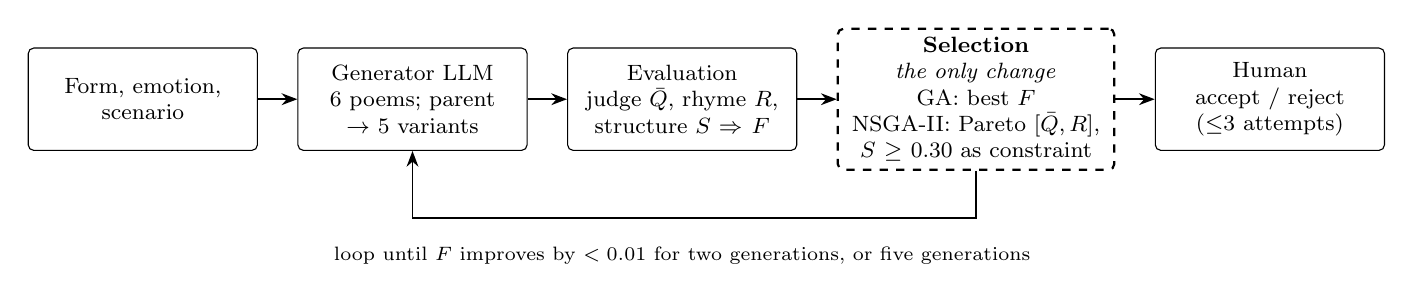
\begin{tikzpicture}[
  box/.style={draw, rounded corners=2pt, align=center, font=\footnotesize,
              minimum height=13mm, text width=27mm, inner sep=3pt, fill=white},
  arr/.style={-{Stealth[length=2mm]}, semithick},
  node distance=5mm]
\node[box] (in) {Form, emotion,\\scenario};
\node[box, right=of in] (gen) {Generator LLM\\6 poems; parent\\$\rightarrow$ 5 variants};
\node[box, right=of gen] (ev) {Evaluation\\judge $\bar Q$, rhyme $R$,\\structure $S$ $\Rightarrow F$};
\node[box, right=of ev, dashed, thick, text width=33mm] (sel) {\textbf{Selection}\\\emph{the only change}\\GA: best $F$\\NSGA-II: Pareto $[\bar Q,R]$,\\$S\ge0.30$ as constraint};
\node[box, right=of sel] (hu) {Human\\accept / reject\\($\le$3 attempts)};
\node[fit=(sel), inner sep=0pt] {};
\draw[arr] (in)--(gen); \draw[arr] (gen)--(ev); \draw[arr] (ev)--(sel); \draw[arr] (sel)--(hu);
\draw[arr] (sel.south) -- ++(0,-6mm) -| (gen.south);
\node[font=\scriptsize, anchor=north] at ($(ev.south)+(0,-11mm)$) {loop until $F$ improves by $<0.01$ for two generations, or five generations};
\end{tikzpicture}
\caption{Overall pipeline. Both algorithms share every stage except selection.}
\label{fig:arch}
\end{figure*}

\textbf{Fitness.} The judge returns five integer sub-scores $q_1,\dots,q_5\in\{1,\dots,5\}$. With $\Qb=\big(\tfrac15\sum_j q_j-1\big)/4$,
\begin{equation}
F = 0.5\,\Qb + 0.25\,R + 0.25\,S .
\label{eq:f}
\end{equation}
$R$ is the rhyme score (AABBA for limericks; haiku start from a $0.5$ baseline since rhyme is optional) and $S$ the syllable-structure score, both computed from the CMU Pronouncing Dictionary \cite{cmudict}. $\Qb$ takes only 21 values, in steps of $0.05$, and the judge is not shown the scenario.

\textbf{Algorithms.} The \emph{GA} is elitist and mutation-only, keeping the best individual by $F$. \emph{NSGA-II} \cite{deb2002} sorts on $[\Qb,R]$ by non-domination and treats $S\ge0.30$ as a feasibility constraint \cite{deb2000constraint}, mutating one parent per generation. Because NSGA-II does not optimise $S$ above the threshold while $S$ carries a quarter of $F$, the scalar $F$ favours the GA by construction; we therefore report $\Qb$ and $S$ separately.

\textbf{Models.} Generator \texttt{openai/\allowbreak gpt-oss-120b} \cite{openai2025gptoss}; judge \texttt{qwen/\allowbreak qwen3.8-27b} \cite{qwen2026}; both served through Groq. All settings were held constant across the twelve accepted runs.

% =====================================================================
\section{Experiments and Results}
% =====================================================================
\textbf{Design.} The design is a full factorial of 2 forms $\times$ 3 emotions $\times$ 2 algorithms, one run per cell; both arms of a cell receive the same scenario, so each cell is a matched pair. Eleven of the twelve poems were accepted on the first attempt; the exception is discussed in Section~\ref{sec:audit}. Across all 13 runs (12 accepted, one rejected attempt), 283 candidate poems were evaluated. One run per cell is a consequence of free-tier rate limits and is the study's main limitation.

\textbf{A scoring defect.} An audit found that the tokeniser pattern \verb|[a-zA-Z']+| matches only the straight apostrophe, so a word written with a typographic one (\textit{Memory's}) splits in two and gains a phantom syllable. Of the 283 candidates, 58 contained one; two of the twelve final poems were affected and are re-scored offline from the logged text (Table~\ref{tab:res}); no logged value was altered. The correction turned one NSGA-II win into a GA win and another cell into an exact tie. Its effect inside the search, where a mis-scored candidate may have changed which parent was selected, cannot be undone offline.

\begin{table}[t]
\caption{Final fitness per condition (one run per cell). $F_c$ is $F$ re-scored for the apostrophe defect; $^\dagger$ marks the two changed poems (GA limerick/sorrow $0.8710\to0.8792$; NSGA-II haiku/sorrow $0.8206\to0.8353$).}
\label{tab:res}
\footnotesize
\begin{tabular}{llcccc}
\toprule
 & & \multicolumn{2}{c}{GA} & \multicolumn{2}{c}{NSGA-II} \\
\cmidrule(lr){3-4}\cmidrule(lr){5-6}
Form & Emotion & $\Qb$ & $F_c$ & $\Qb$ & $F_c$ \\
\midrule
Limerick & Fear   & 0.85 & 0.8798 & 0.90 & 0.9106 \\
Limerick & Joy    & 0.85 & 0.8516 & 0.80 & 0.8070 \\
Limerick & Sorrow & 0.90 & 0.8792$^\dagger$ & 0.90 & 0.8766 \\
Haiku    & Fear   & 0.85 & 0.8000 & 0.85 & 0.7853 \\
Haiku    & Joy    & 0.80 & 0.7750 & 0.85 & 0.8000 \\
Haiku    & Sorrow & 0.95 & 0.8353 & 0.95 & 0.8353$^\dagger$ \\
\midrule
\multicolumn{2}{l}{Mean} & 0.867 & 0.8368 & 0.875 & 0.8358 \\
\bottomrule
\end{tabular}
\end{table}

\begin{figure}[t]
\centering
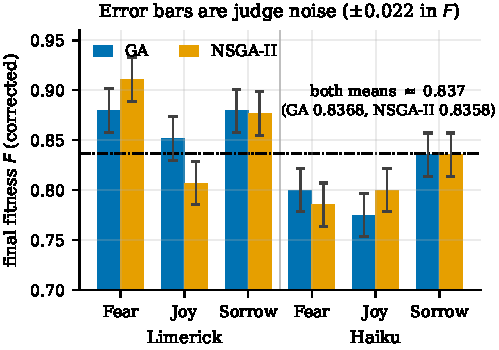
\includegraphics[width=\columnwidth]{fig_ga_vs_nsga.pdf}
\caption{Final fitness by condition. Error bars show judge noise ($\pm0.0218$ in $F$, Section~\ref{sec:audit}); the full span of a bar (0.044) exceeds every between-algorithm gap except the largest (0.0446).}
\label{fig:ga}
\end{figure}

\textbf{RQ1: no evidence of a difference.} Mean final $F$ is $0.8368$ (GA) against $0.8358$ (NSGA-II), a difference of $0.0010$ ($0.0021$ uncorrected, same direction). The GA wins three cells, NSGA-II two, and one is an exact tie. An exact two-sided Wilcoxon signed-rank test, run on the five untied pairs, gives $p=1.0$ but has almost no power: with five pairs the smallest attainable two-sided $p$ is $0.0625$, so even unanimity could not have reached $0.05$. The accurate reading is not that the test found no difference but that six pairs cannot show one. By term, NSGA-II is marginally ahead on $\Qb$ ($0.875$ vs.\ $0.867$; two wins, one loss, three ties) and the GA on $S$ ($0.858$ vs.\ $0.833$), as the constraint design predicts; both gaps are small (the $\Qb$ gap is a sixth of one judge step) and untested. Wall-clock time is dominated by rate-limit waits, and token use per run is similar across arms.

% =====================================================================
\section{Auditing the Fitness Function}\label{sec:audit}
% =====================================================================
A null result is uninformative if the fitness function cannot discriminate. We scored 53 poems with the same judge model and one shared four-dimension rubric (imagery, literary devices, originality, coherence), three times each (159 calls): (A) 30 published human poems (15 haiku; 15 English limericks, mostly by Lear), (B) 10 deliberately bad controls that keep correct form, and (C) the 13 evolved poems. Group~A is reported in aggregate only.

\begin{figure}[t]
\centering
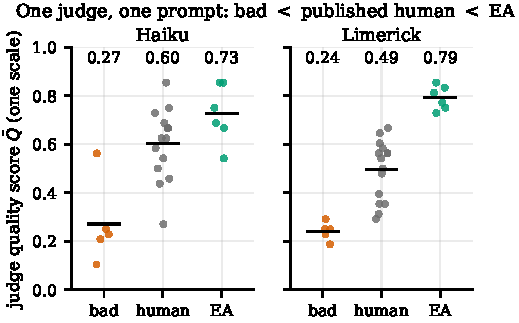
\includegraphics[width=\columnwidth]{fig_judge_groups.pdf}
\caption{Per-poem mean judge score by group on one scale: bad $<$ published human $<$ evolved, in both forms. Bars are group means.}
\label{fig:groups}
\end{figure}


\begin{table}[t]
\caption{Judge sub-score means (1--5) for limericks, evolved ($n{=}6$) vs.\ published human ($n{=}15$). Differences use unrounded means.}
\label{tab:dims}
\footnotesize
\begin{tabular}{lccc}
\toprule
Dimension & Evolved & Human & Diff. \\
\midrule
Imagery          & 4.33 & 2.98 & $+1.36$ \\
Literary devices & 4.11 & 2.29 & $+1.82$ \\
Originality      & 3.50 & 1.91 & $+1.59$ \\
Coherence        & 4.72 & 4.73 & $-0.01$ \\
\bottomrule
\end{tabular}
\end{table}

\textbf{RQ2: it discriminates, but prefers ornament.} Figure~\ref{fig:groups} shows the ordering. Human poems beat the bad controls (haiku $0.604$ vs.\ $0.271$, $p=0.005$; limerick $0.494$ vs.\ $0.242$, $p=0.001$; Mann--Whitney $U$ \cite{mann1947} on per-poem means), so the fitness function is not noise. Evolved poems also outscore human ones: haiku $0.726$ vs.\ $0.604$ ($p=0.078$) and limerick $0.792$ vs.\ $0.494$ ($p=0.0005$), with all six evolved limericks above all fifteen canonical ones. Coherence is identical ($4.72$ vs.\ $4.73$); the gap is imagery ($+1.36$), literary devices ($+1.82$) and originality ($+1.59$) (Table~\ref{tab:dims}). A Lear limerick is deliberately plain, and the rubric has no dimension for humour or comic timing, so it scores what the form is built on at zero weight and rewards ornament. This is a property of the rubric, hence fixable, and the comparison with human limericks is evidence about the judge, not about the poems.


\begin{figure}[t]
\centering
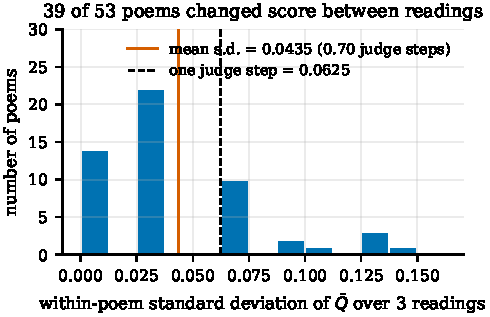
\includegraphics[width=\columnwidth]{fig_judge_noise.pdf}
\caption{Spread of the three readings of each poem. Most poems do not receive the same score twice; the mean spread is close to one judge step.}
\label{fig:noise}
\end{figure}

\textbf{RQ3: it is unstable.} Of the 53 poems, 39 ($73.6\%$) changed score between identical readings (Figure~\ref{fig:noise}); the mean within-poem standard deviation is $0.0435$ ($0.70$ of a judge step), and the worst poem has a range of $0.25$. One reading carries weight $0.5$ in Eq.~\ref{eq:f}, so this is $\pm0.0218$ in $F$: about twenty times the $0.0010$ gap. The standard deviation of a GA-minus-NSGA-II difference from judge noise alone ($0.031$) exceeds four of the six per-cell gaps and roughly equals a fifth. Detecting an effect of the observed size at $80\%$ power would need on the order of 7{,}000 pairs, so the remedy is a better instrument, not more runs. Averaging $k$ readings cuts noise by $\sqrt k$; three give $\pm0.0126$.

\textbf{A case where fitness was wrong.} The one rejected poem (GA haiku/joy) had higher production fitness than its accepted replacement ($0.7917$ vs.\ $0.7750$), while the calibration judge ranks them the other way ($0.583$ vs.\ $0.667$), agreeing with the human verdict. One case proves nothing but points the same way.

% =====================================================================
\section{Threats to Validity and Next Phase}
% =====================================================================
\textbf{Threats.} One run per cell, so run-to-run variance is not separable. Noise was measured with the four-dimension calibration rubric (step $0.0625$), not the five-dimension production rubric (step $0.05$); we assume comparable noise. One judge family and provider, with biases \cite{zheng2023,wang2024fair} uncontrolled. The only human signal is one accept/reject per run, made by the first author, not blind to condition. The rubric omits humour. The apostrophe defect perturbed the search.

\textbf{Committed protocol.} The fix is implemented behind a single flag: the judge averaged over three readings (unreadable replies skipped, not replaced by a middle score); apostrophe normalisation applied before scoring only; three replicates per cell (36 runs) with a restartable grid; per-candidate logging; Phase~I logs never modified. A live test run confirmed the averaging path; the full grid has not been run and no result from it is claimed. A humour dimension and two NSGA-II quirks (tie-breaking by list order, a best-so-far tracker) are deliberately kept out, so the instrument and the algorithms are not changed in the same step.

% =====================================================================
\section{Conclusion}
% =====================================================================
Given the same generator, judge and budget, we find no evidence that NSGA-II beats an elitist GA (gap $0.0010$; wins split three to two with one tie). More usefully, we show why this could not be settled with this instrument: the judge discriminates but is unstable ($73.6\%$ of poems changed score between identical readings; $\pm0.0218$ in $F$) and prefers ornate writing. Practitioners should report the noise of their judge before the benefit of their algorithm. Code, logs and data: \url{https://github.com/sakthicr/LLMMM}.

\bibliographystyle{ACM-Reference-Format}
\bibliography{refs}

\end{document}
